\documentclass[12pt,a4paper]{article}
\usepackage{solutions}
\usepackage{multicol}
\usepackage{float}
\usepackage{inkscape}

\title{Домашнее задание от 14.09.\\Теоретическая информатика. 2 курс.\\Решения.}
\author{Глеб Минаев @ 204 (20.Б04-мкн)}
% \date{}

\newcommand{\lex}{\mathrm{lex}}

\begin{document}
    \maketitle

    \begin{multicols}{2}
        \tableofcontents
    \end{multicols}

    \begin{problem}{1}\ 
        \begin{figure}[H]
            \centering
            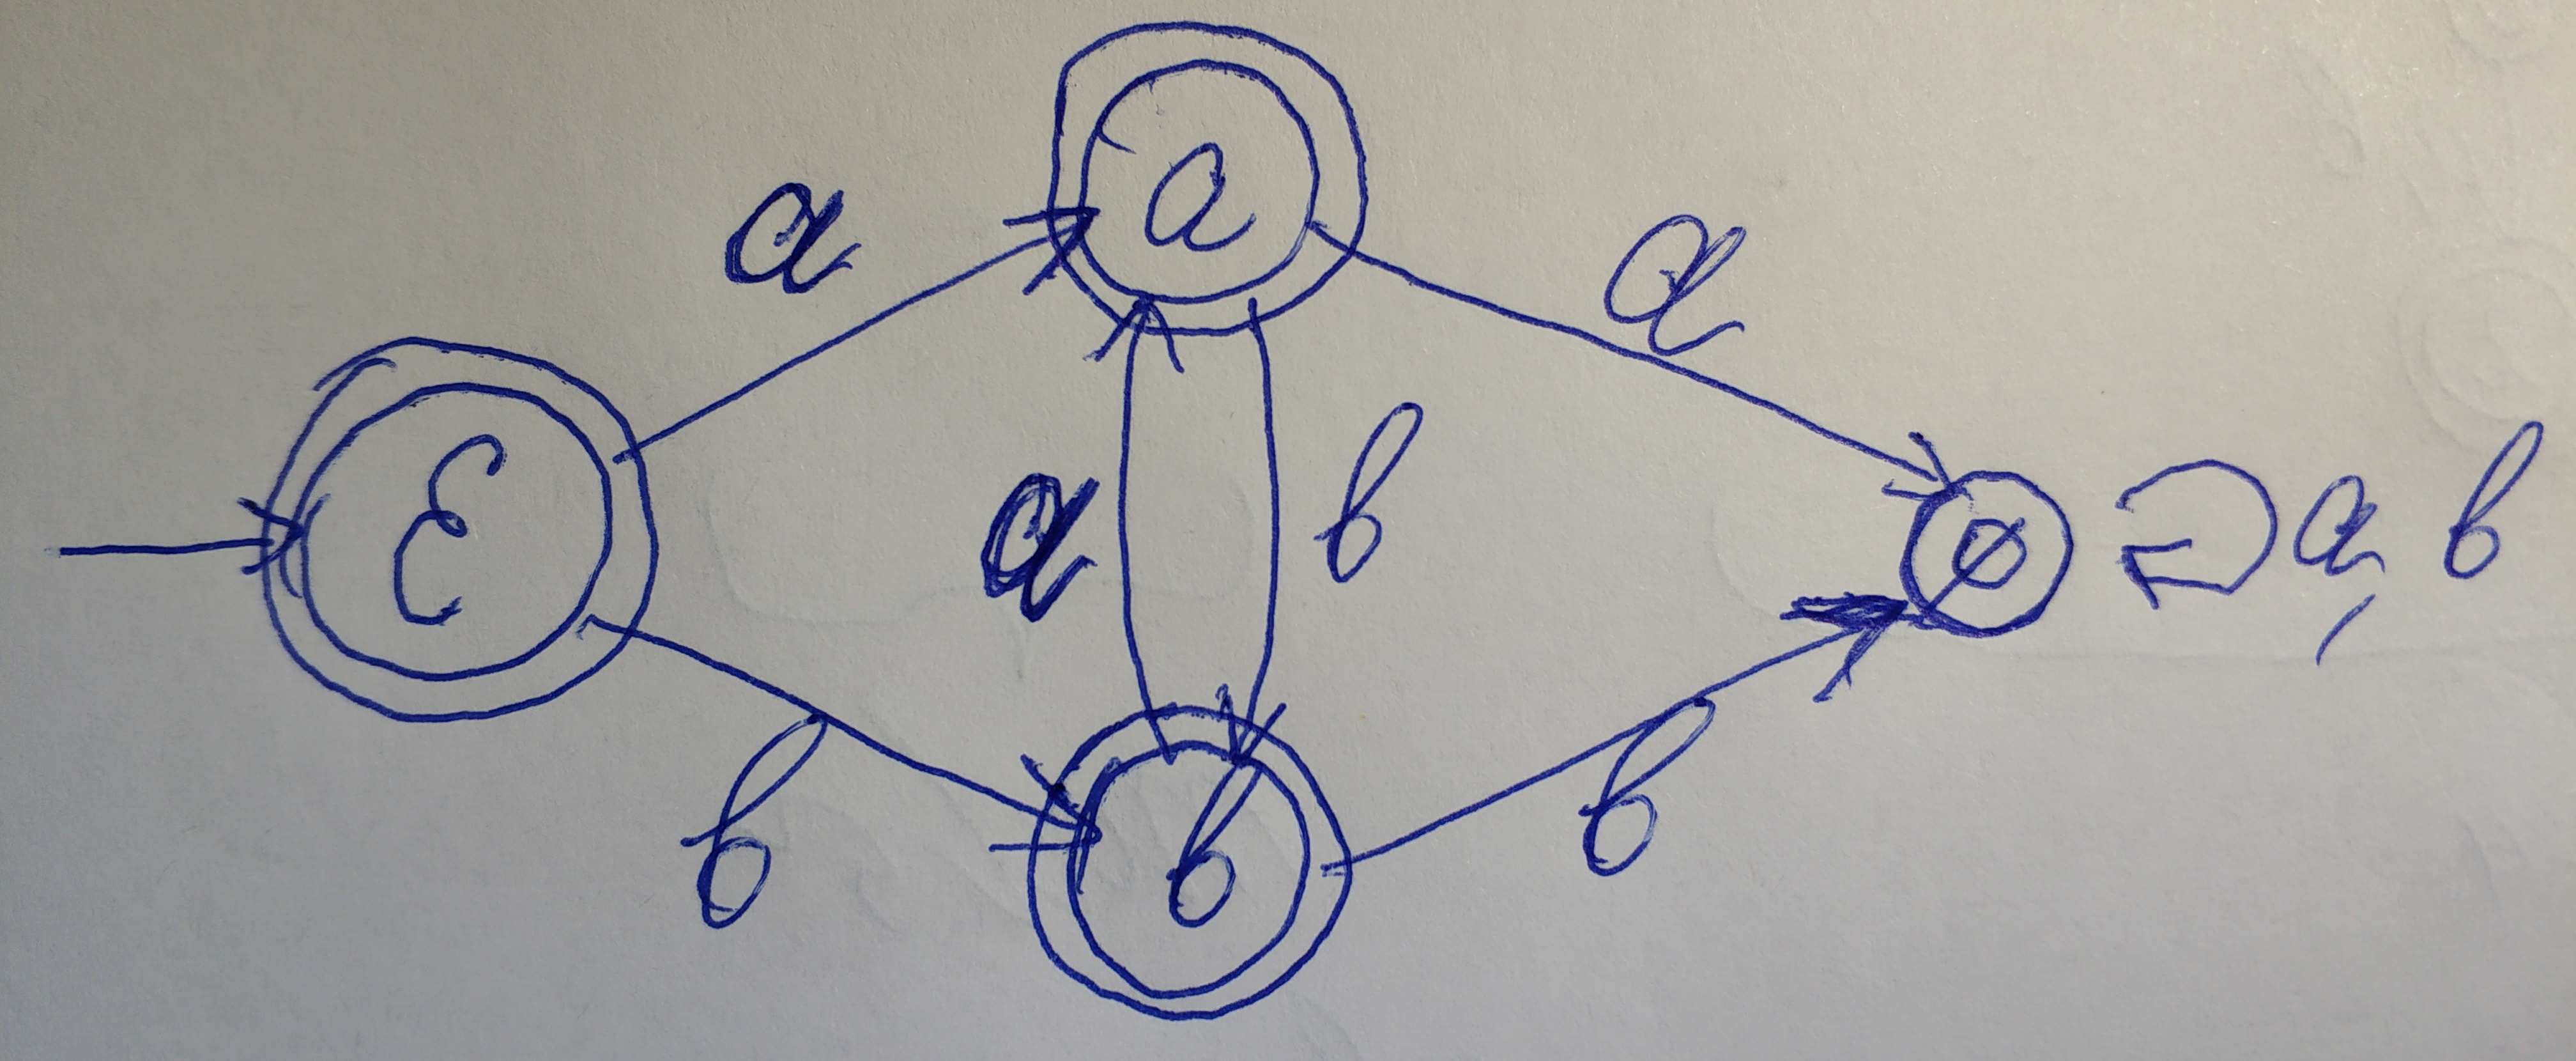
\includegraphics[height=3cm]{TI-HW-002-1.jpg}
            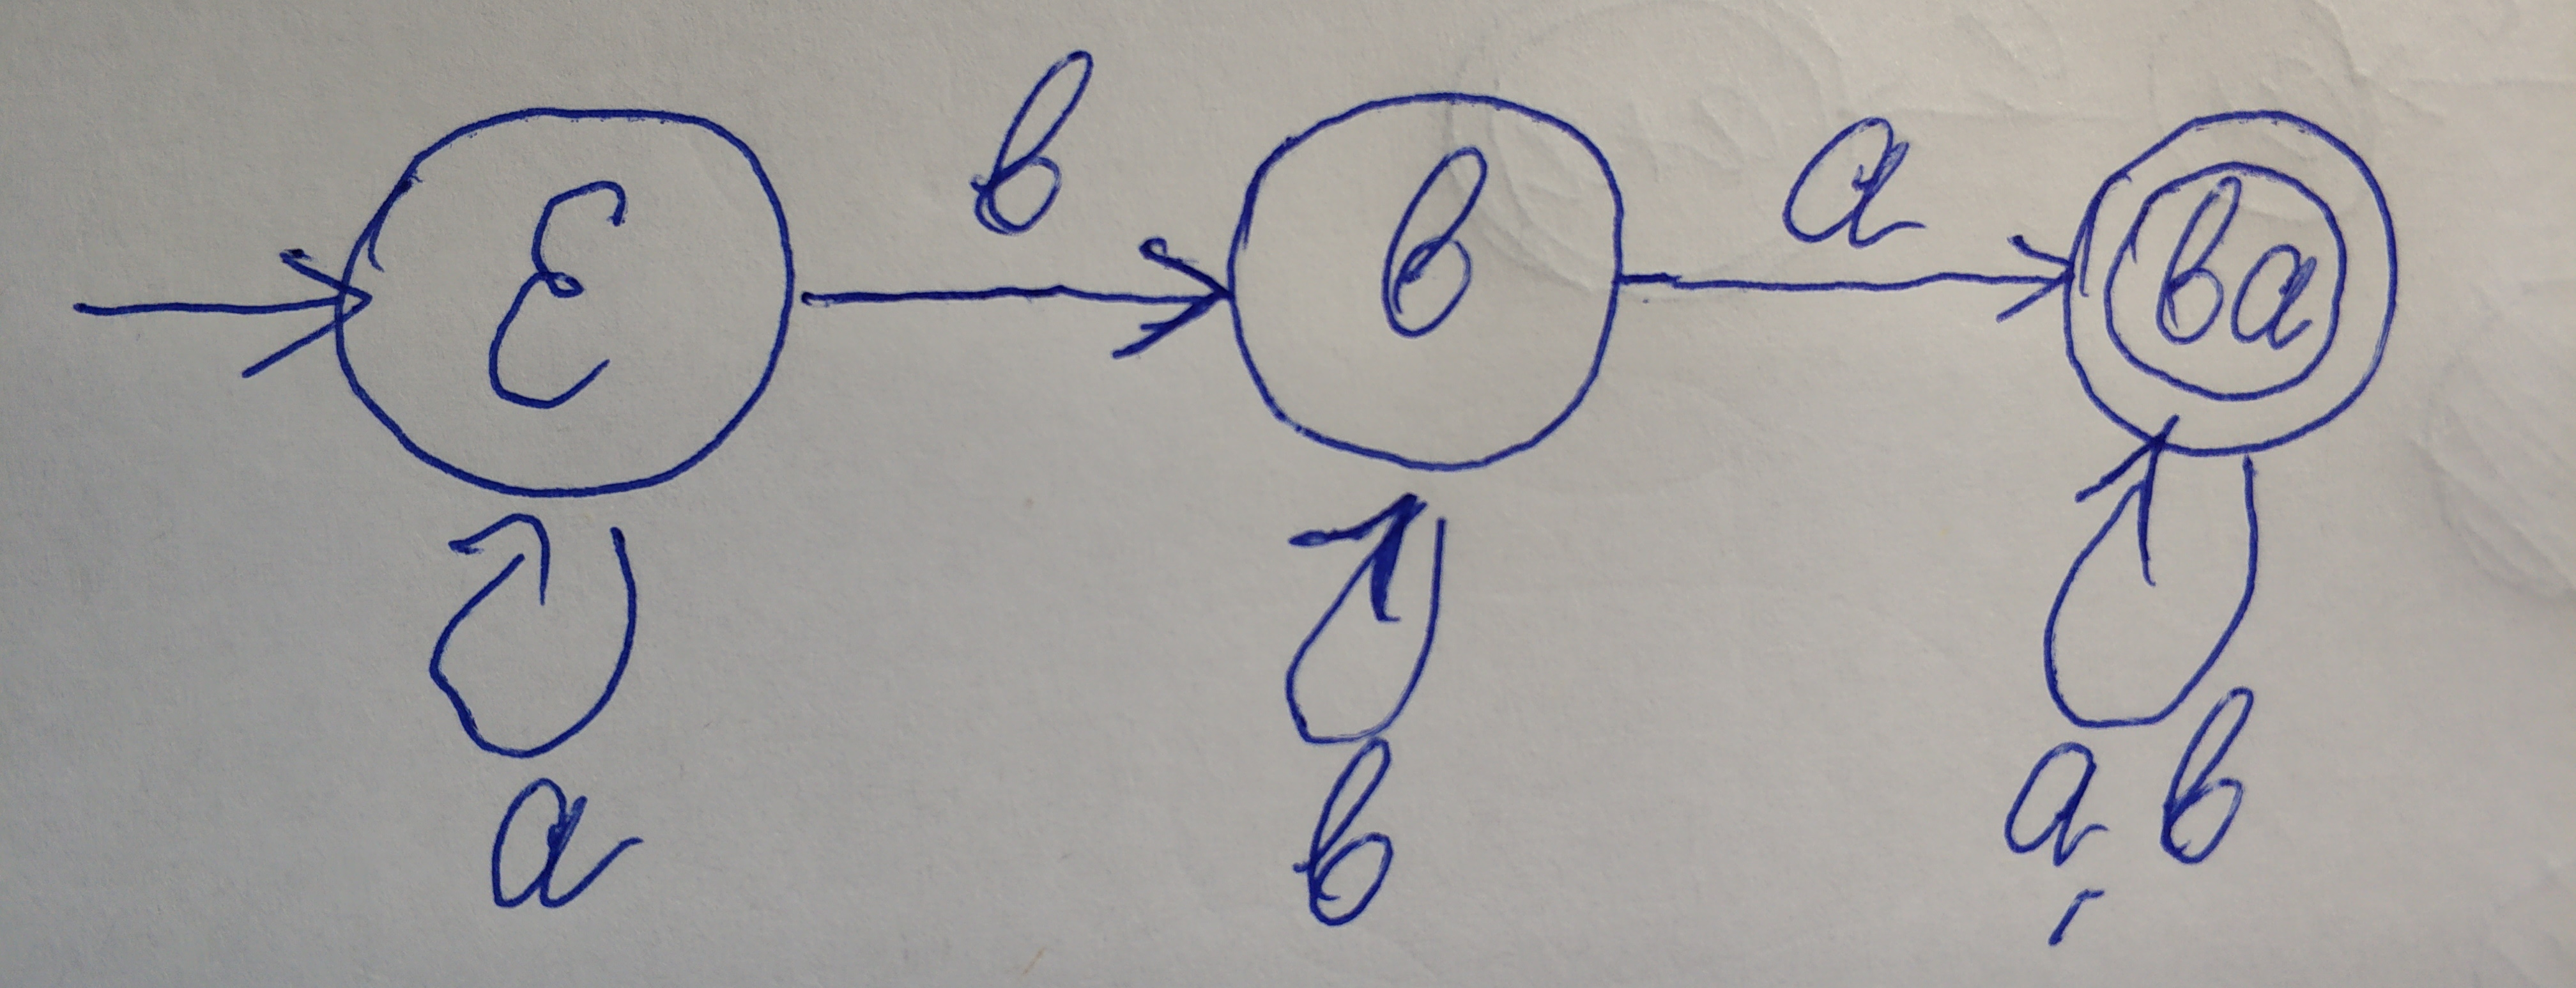
\includegraphics[height=3cm]{TI-HW-002-2.jpg}
        \end{figure}
    \end{problem}

    \begin{problem}{2}\ 
        \begin{figure}[H]
            \centering
            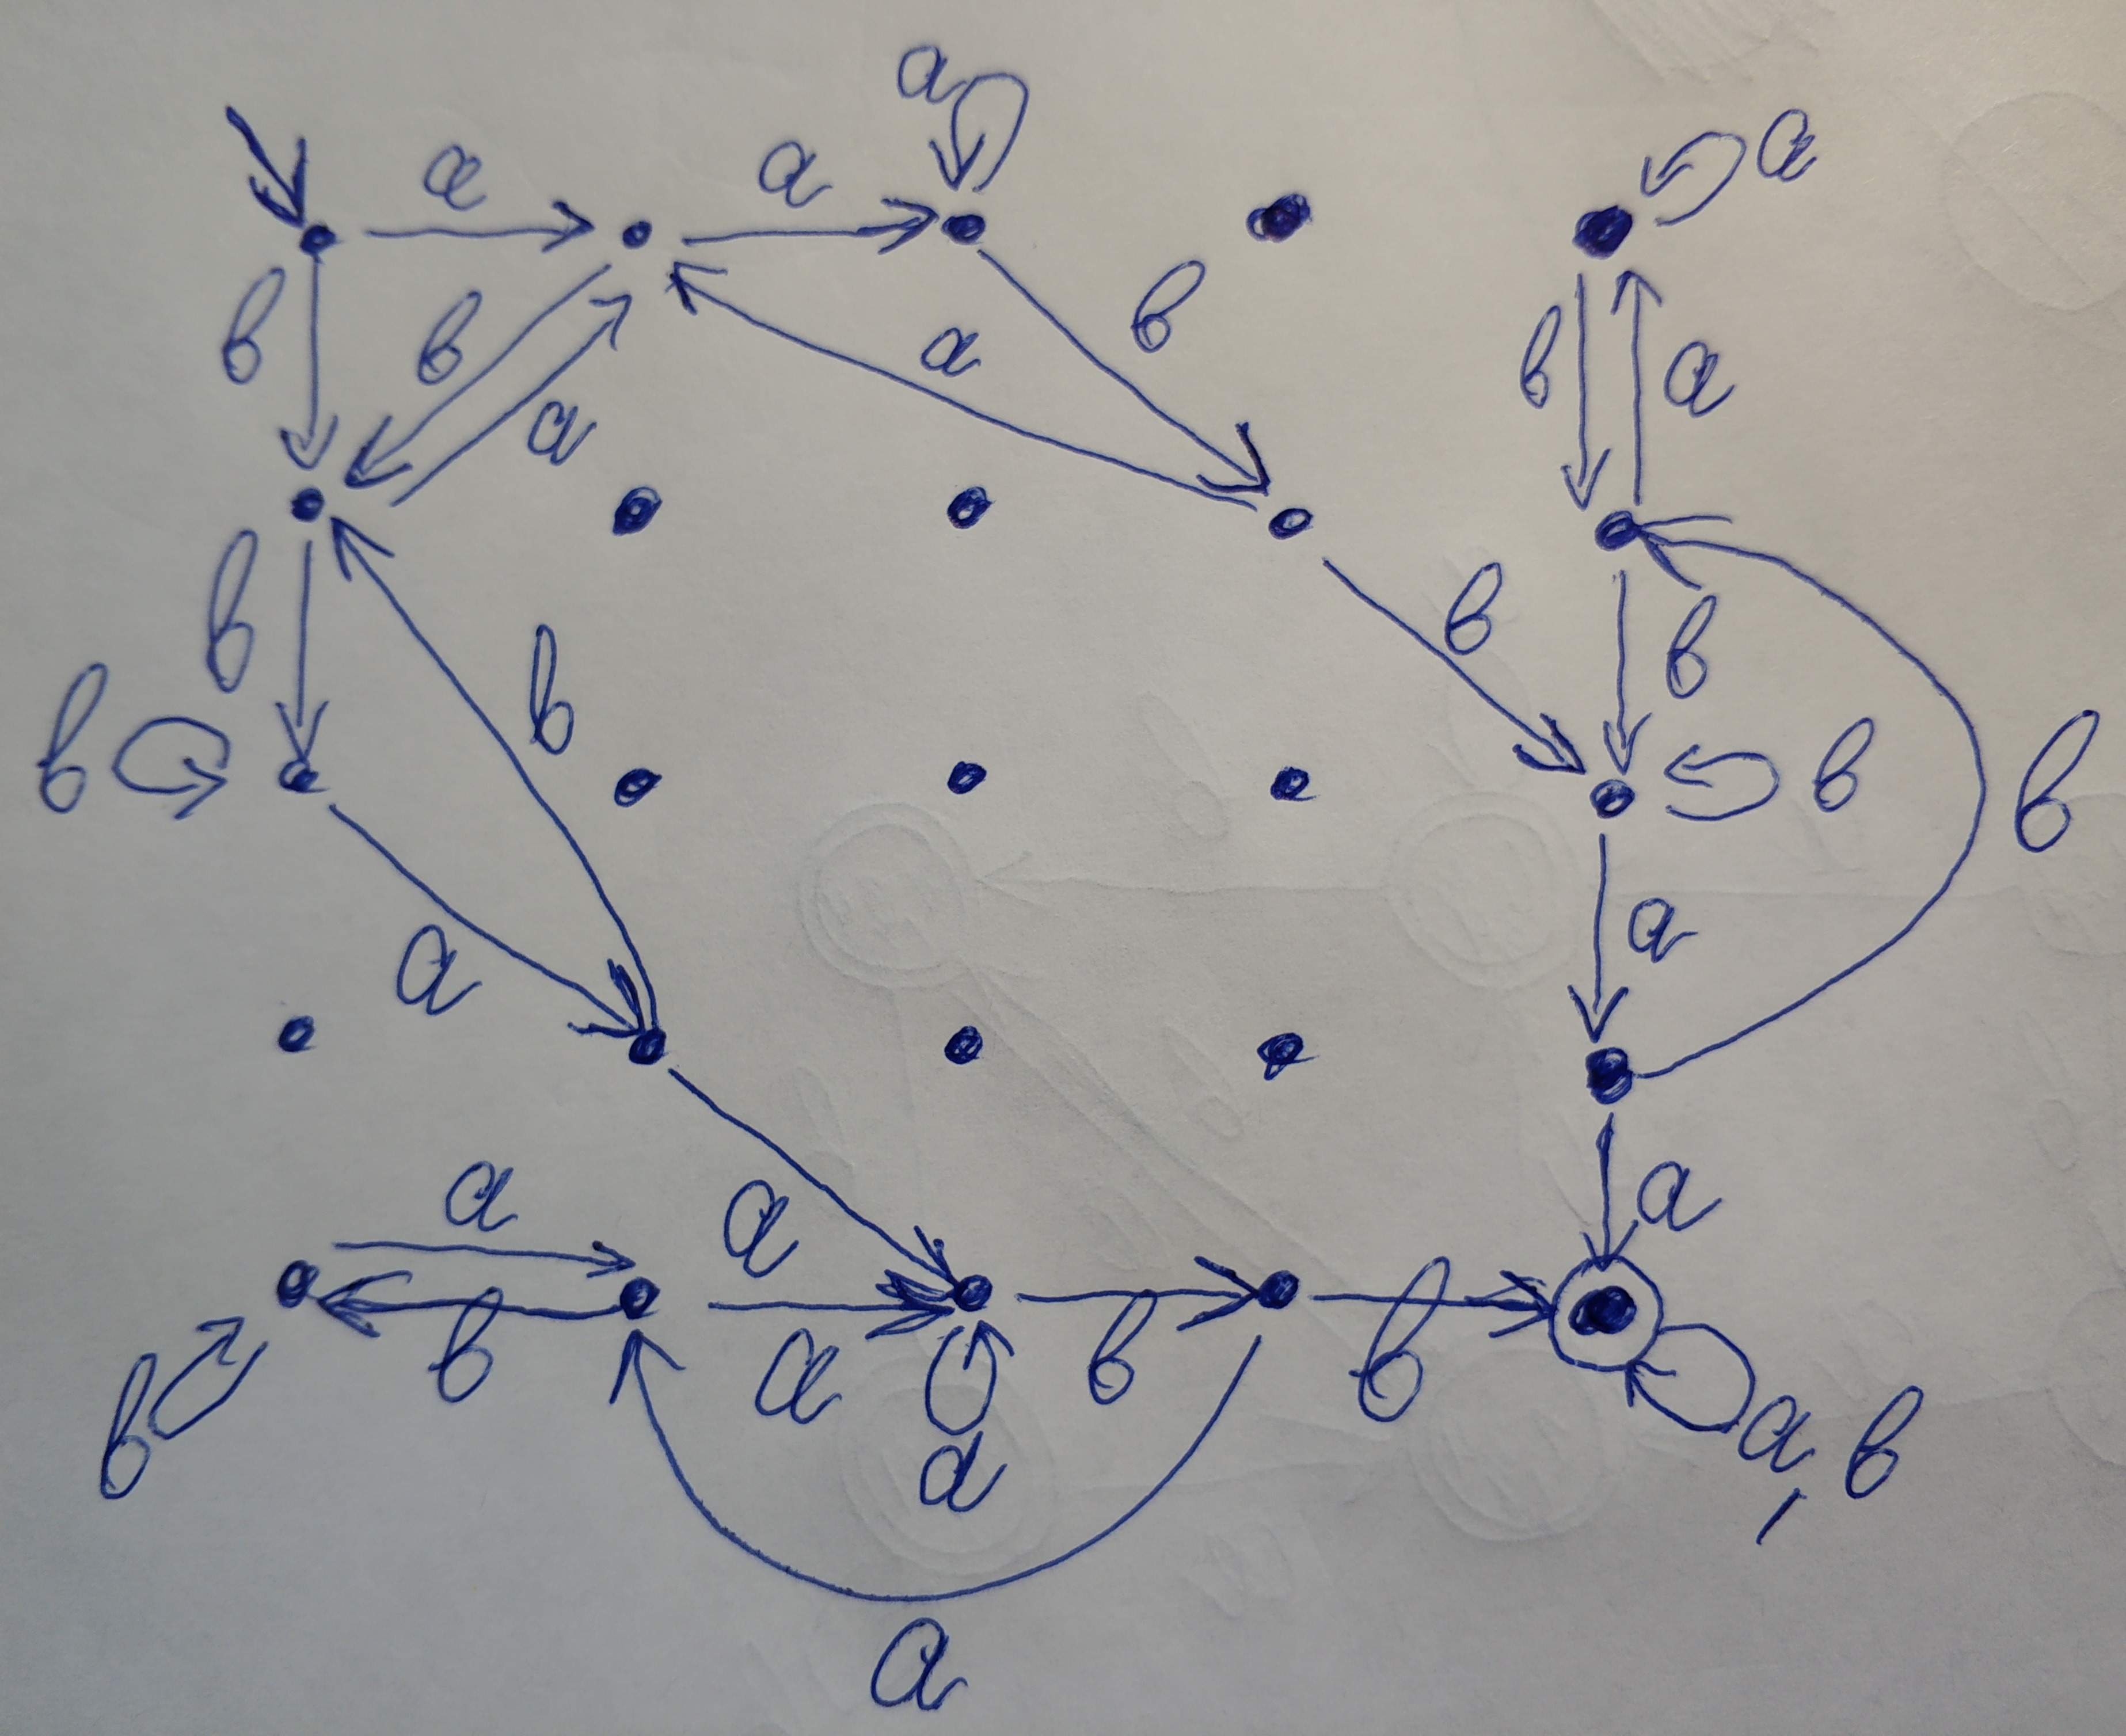
\includegraphics[height=3cm]{TI-HW-002-3.jpg}
            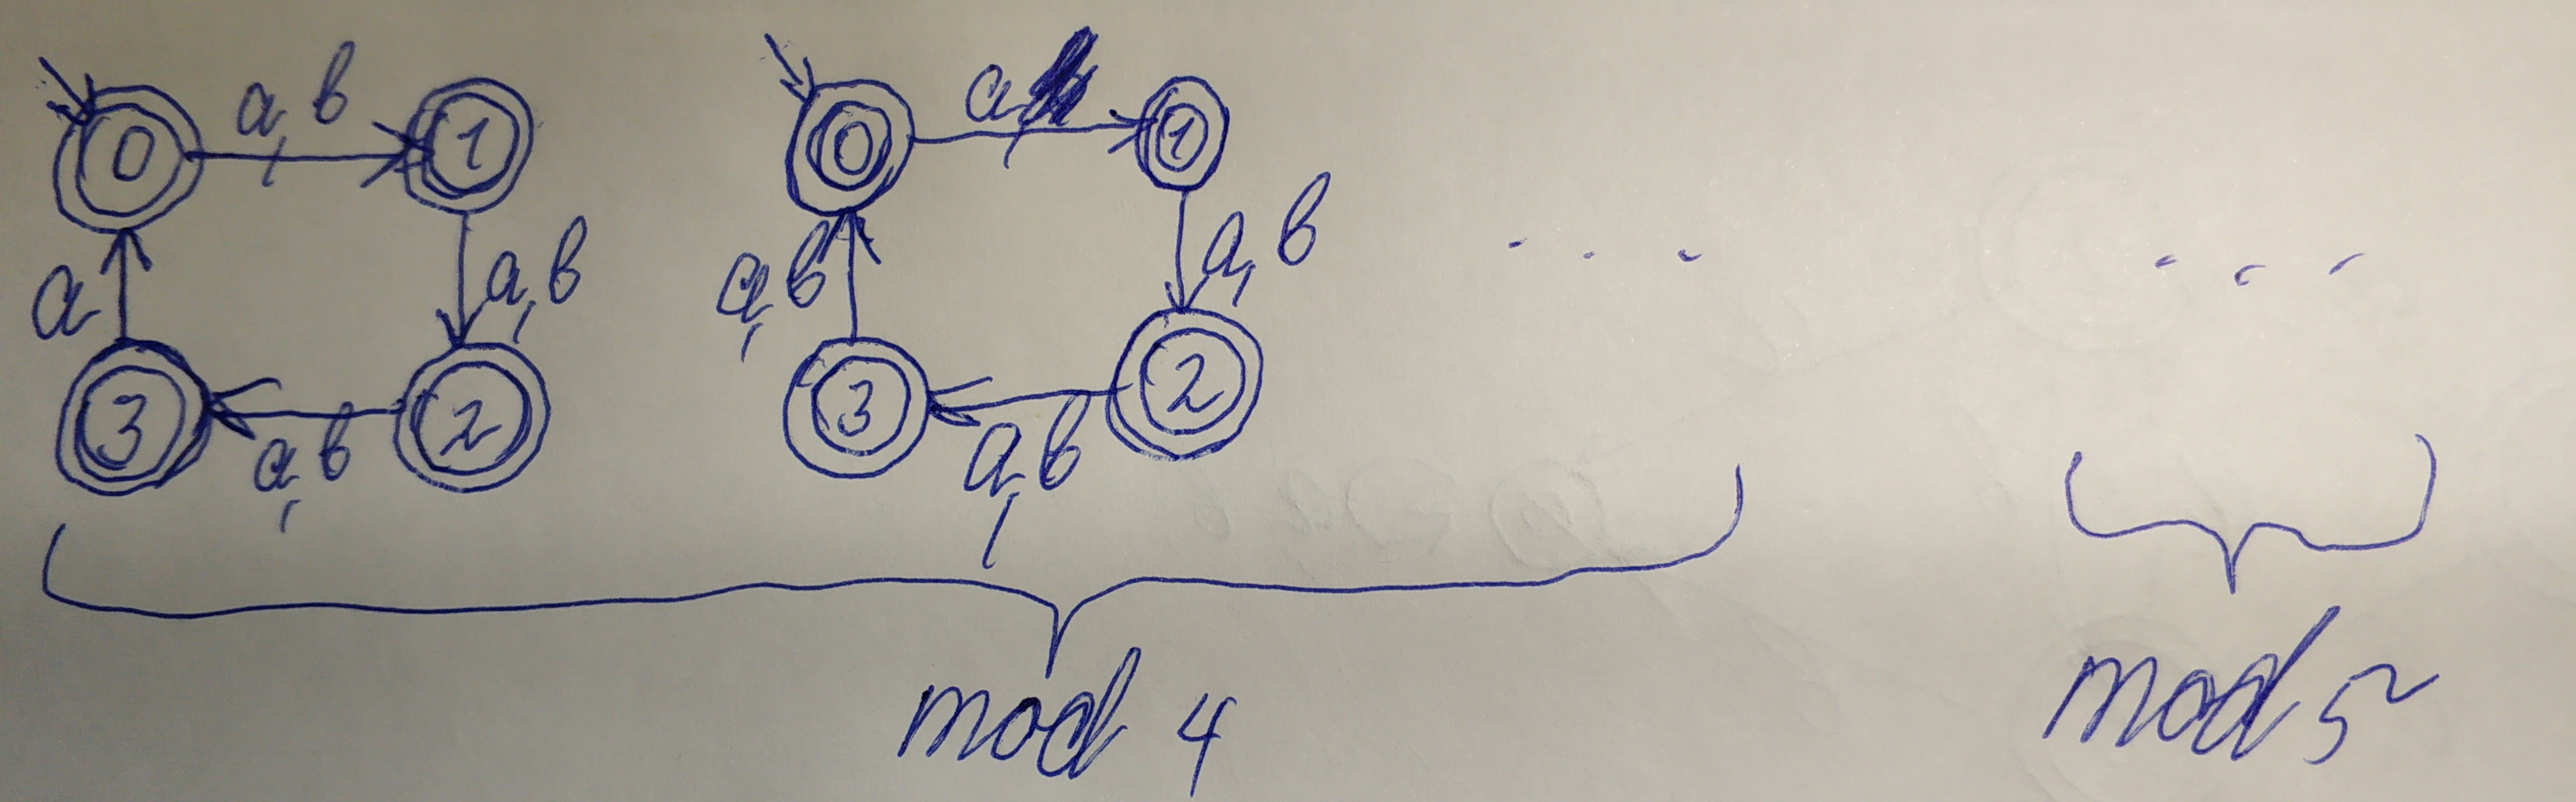
\includegraphics[height=3cm]{TI-HW-002-4.jpg}
        \end{figure}
    \end{problem}

    \begin{problem}{4}\ 
        \begin{figure}[H]
            \centering
            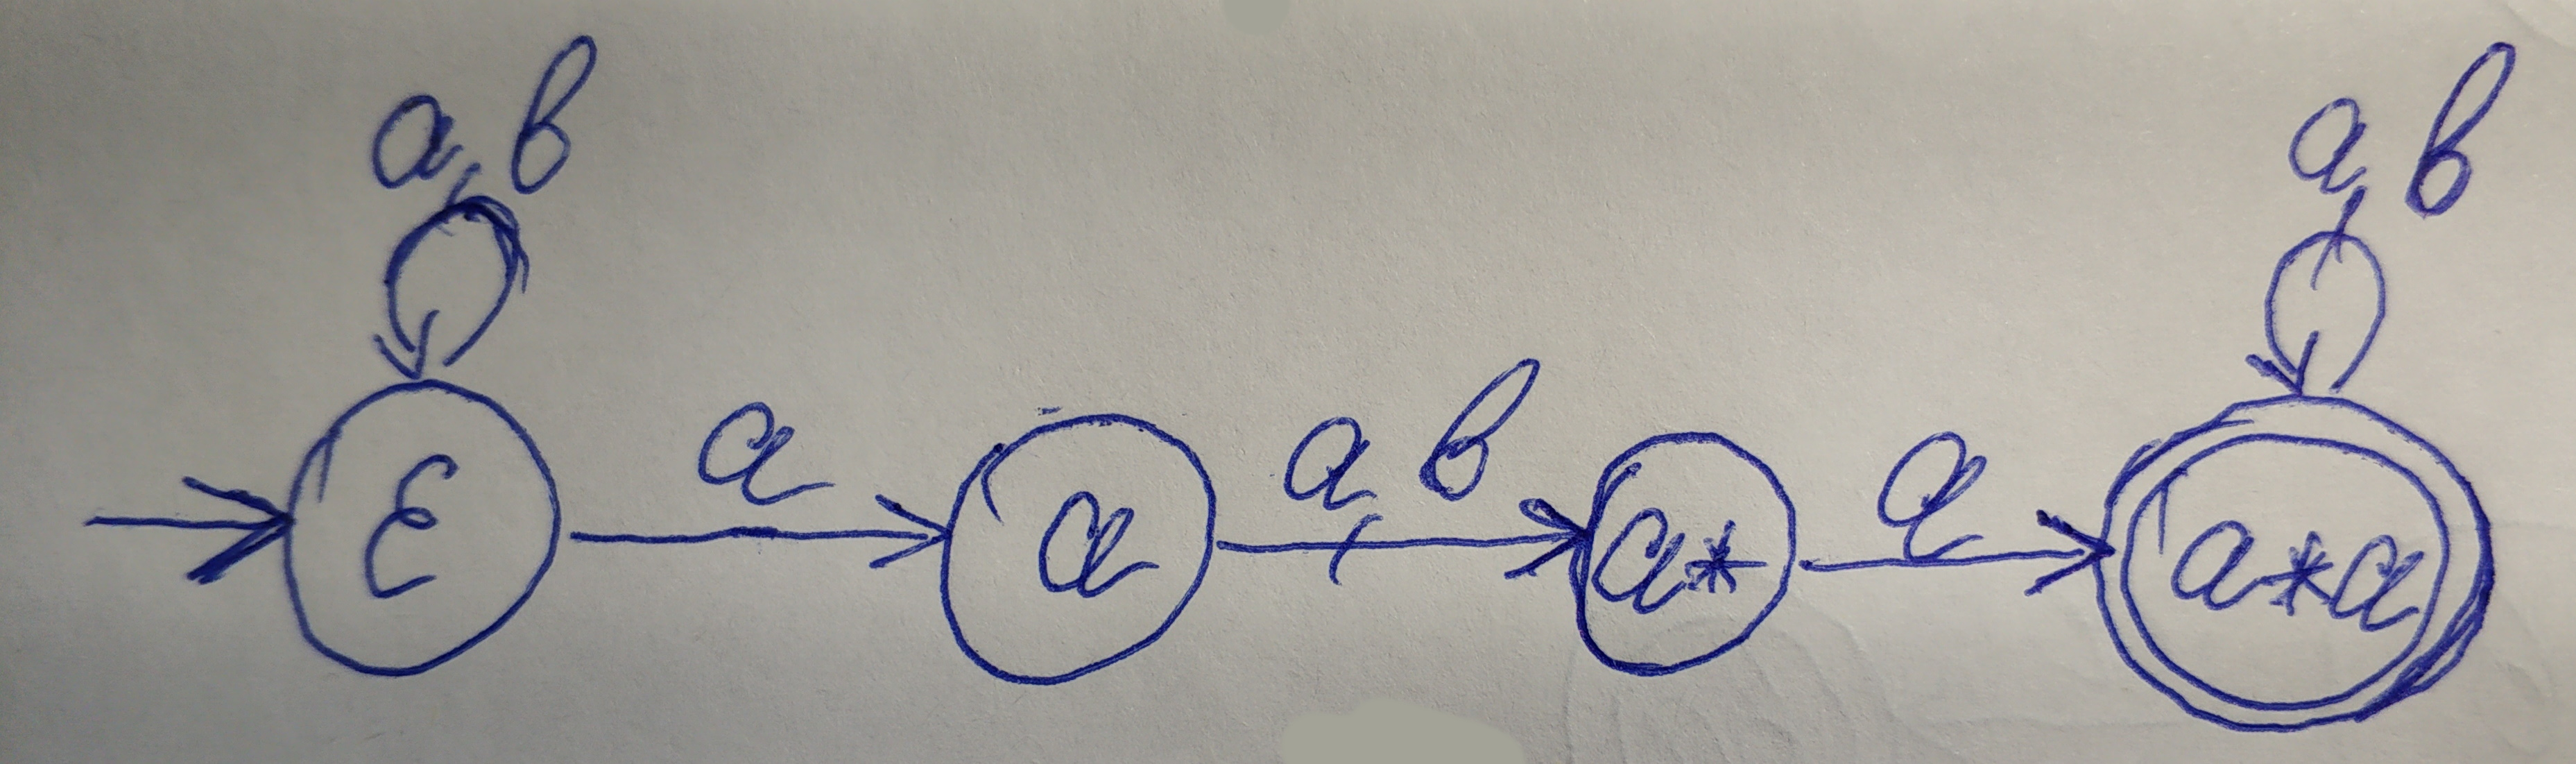
\includegraphics[height=3cm]{TI-HW-002-5.jpg}
            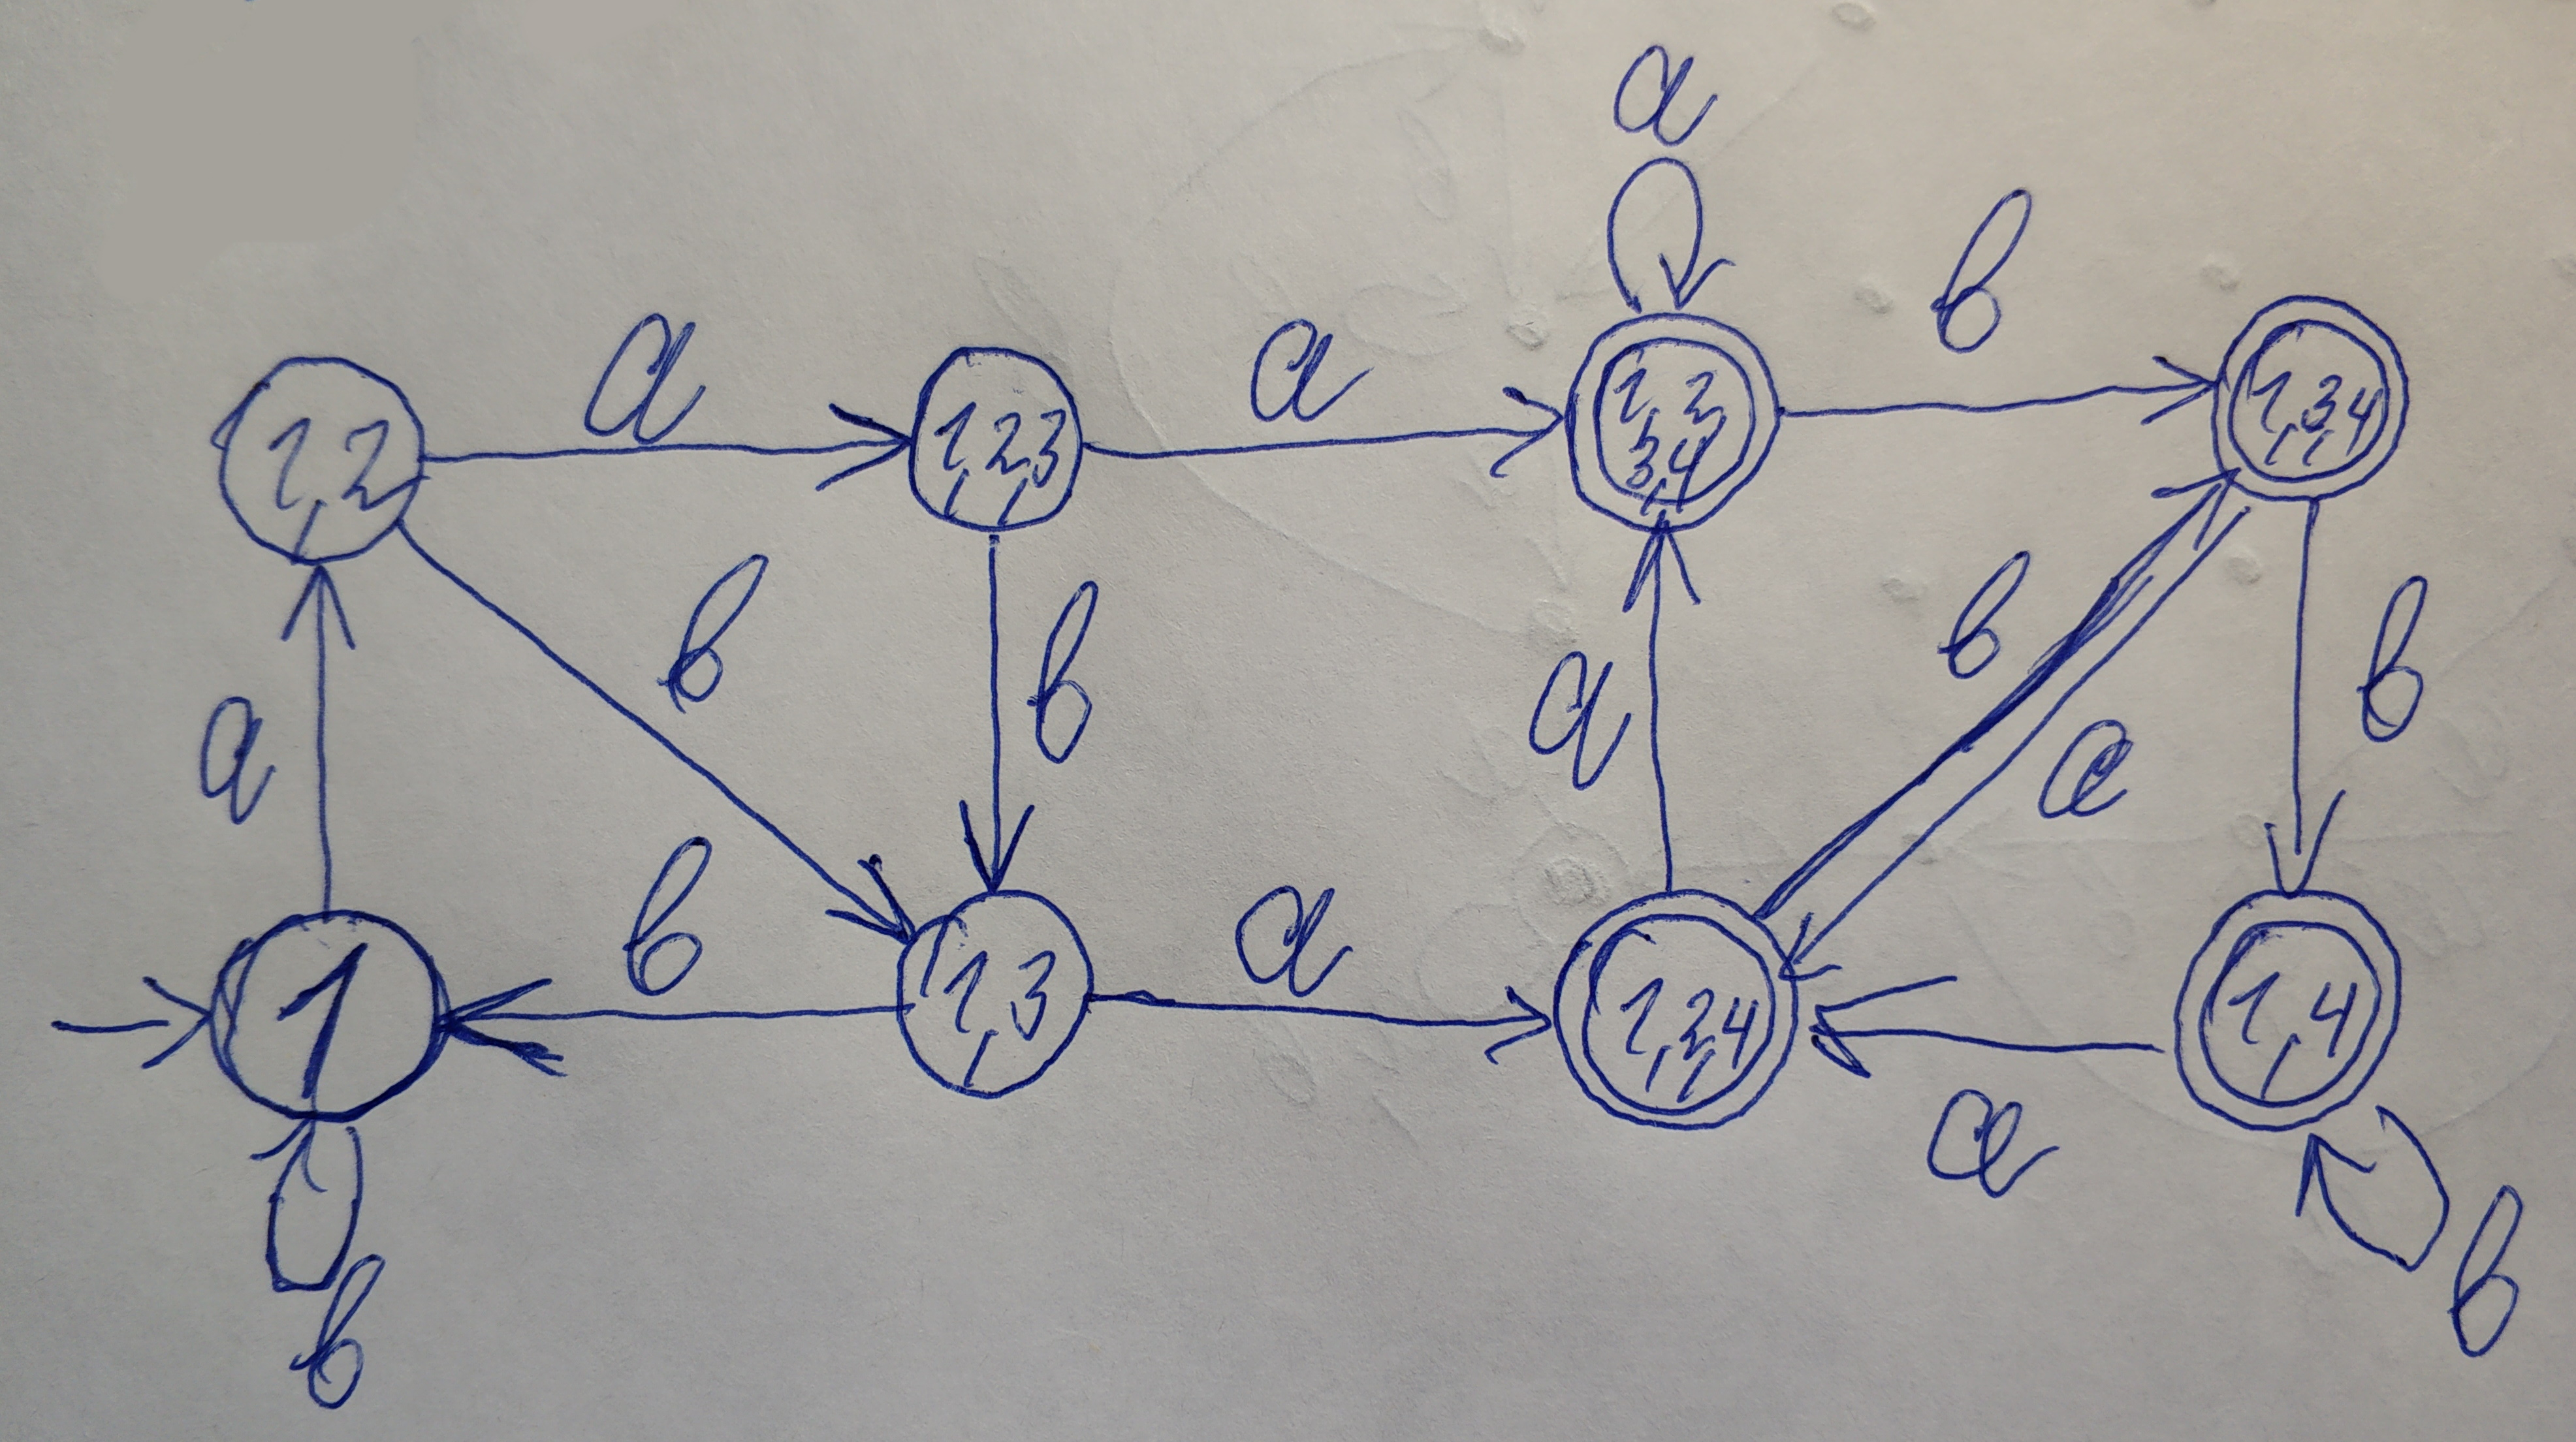
\includegraphics[height=3cm]{TI-HW-002-6.jpg}
        \end{figure}
    \end{problem}

    \begin{problem}{5}
        Рассмотрим язык $L := \{(ab)^n\}_{n \in \NN}$. Заметим, что он регулярный. Например, он распознаётся машиной на рисунке. У неё есть три состояния: ``всё ОК'' (когда прочитанная в данный момент строка соответствует описанию), ``прочитал $a$, жду $b$'' (когда был прочитан ещё один символ $a$, и, соответственно, не хватает символа $b$ до соответствия описанию) и ``точно не подходит'' (прочли что-то странное и подогнать результат под описание уже невозможно). Переходы между состояниями понятным образом выходят из описания состояний.
        \begin{figure}[H]
            \centering
            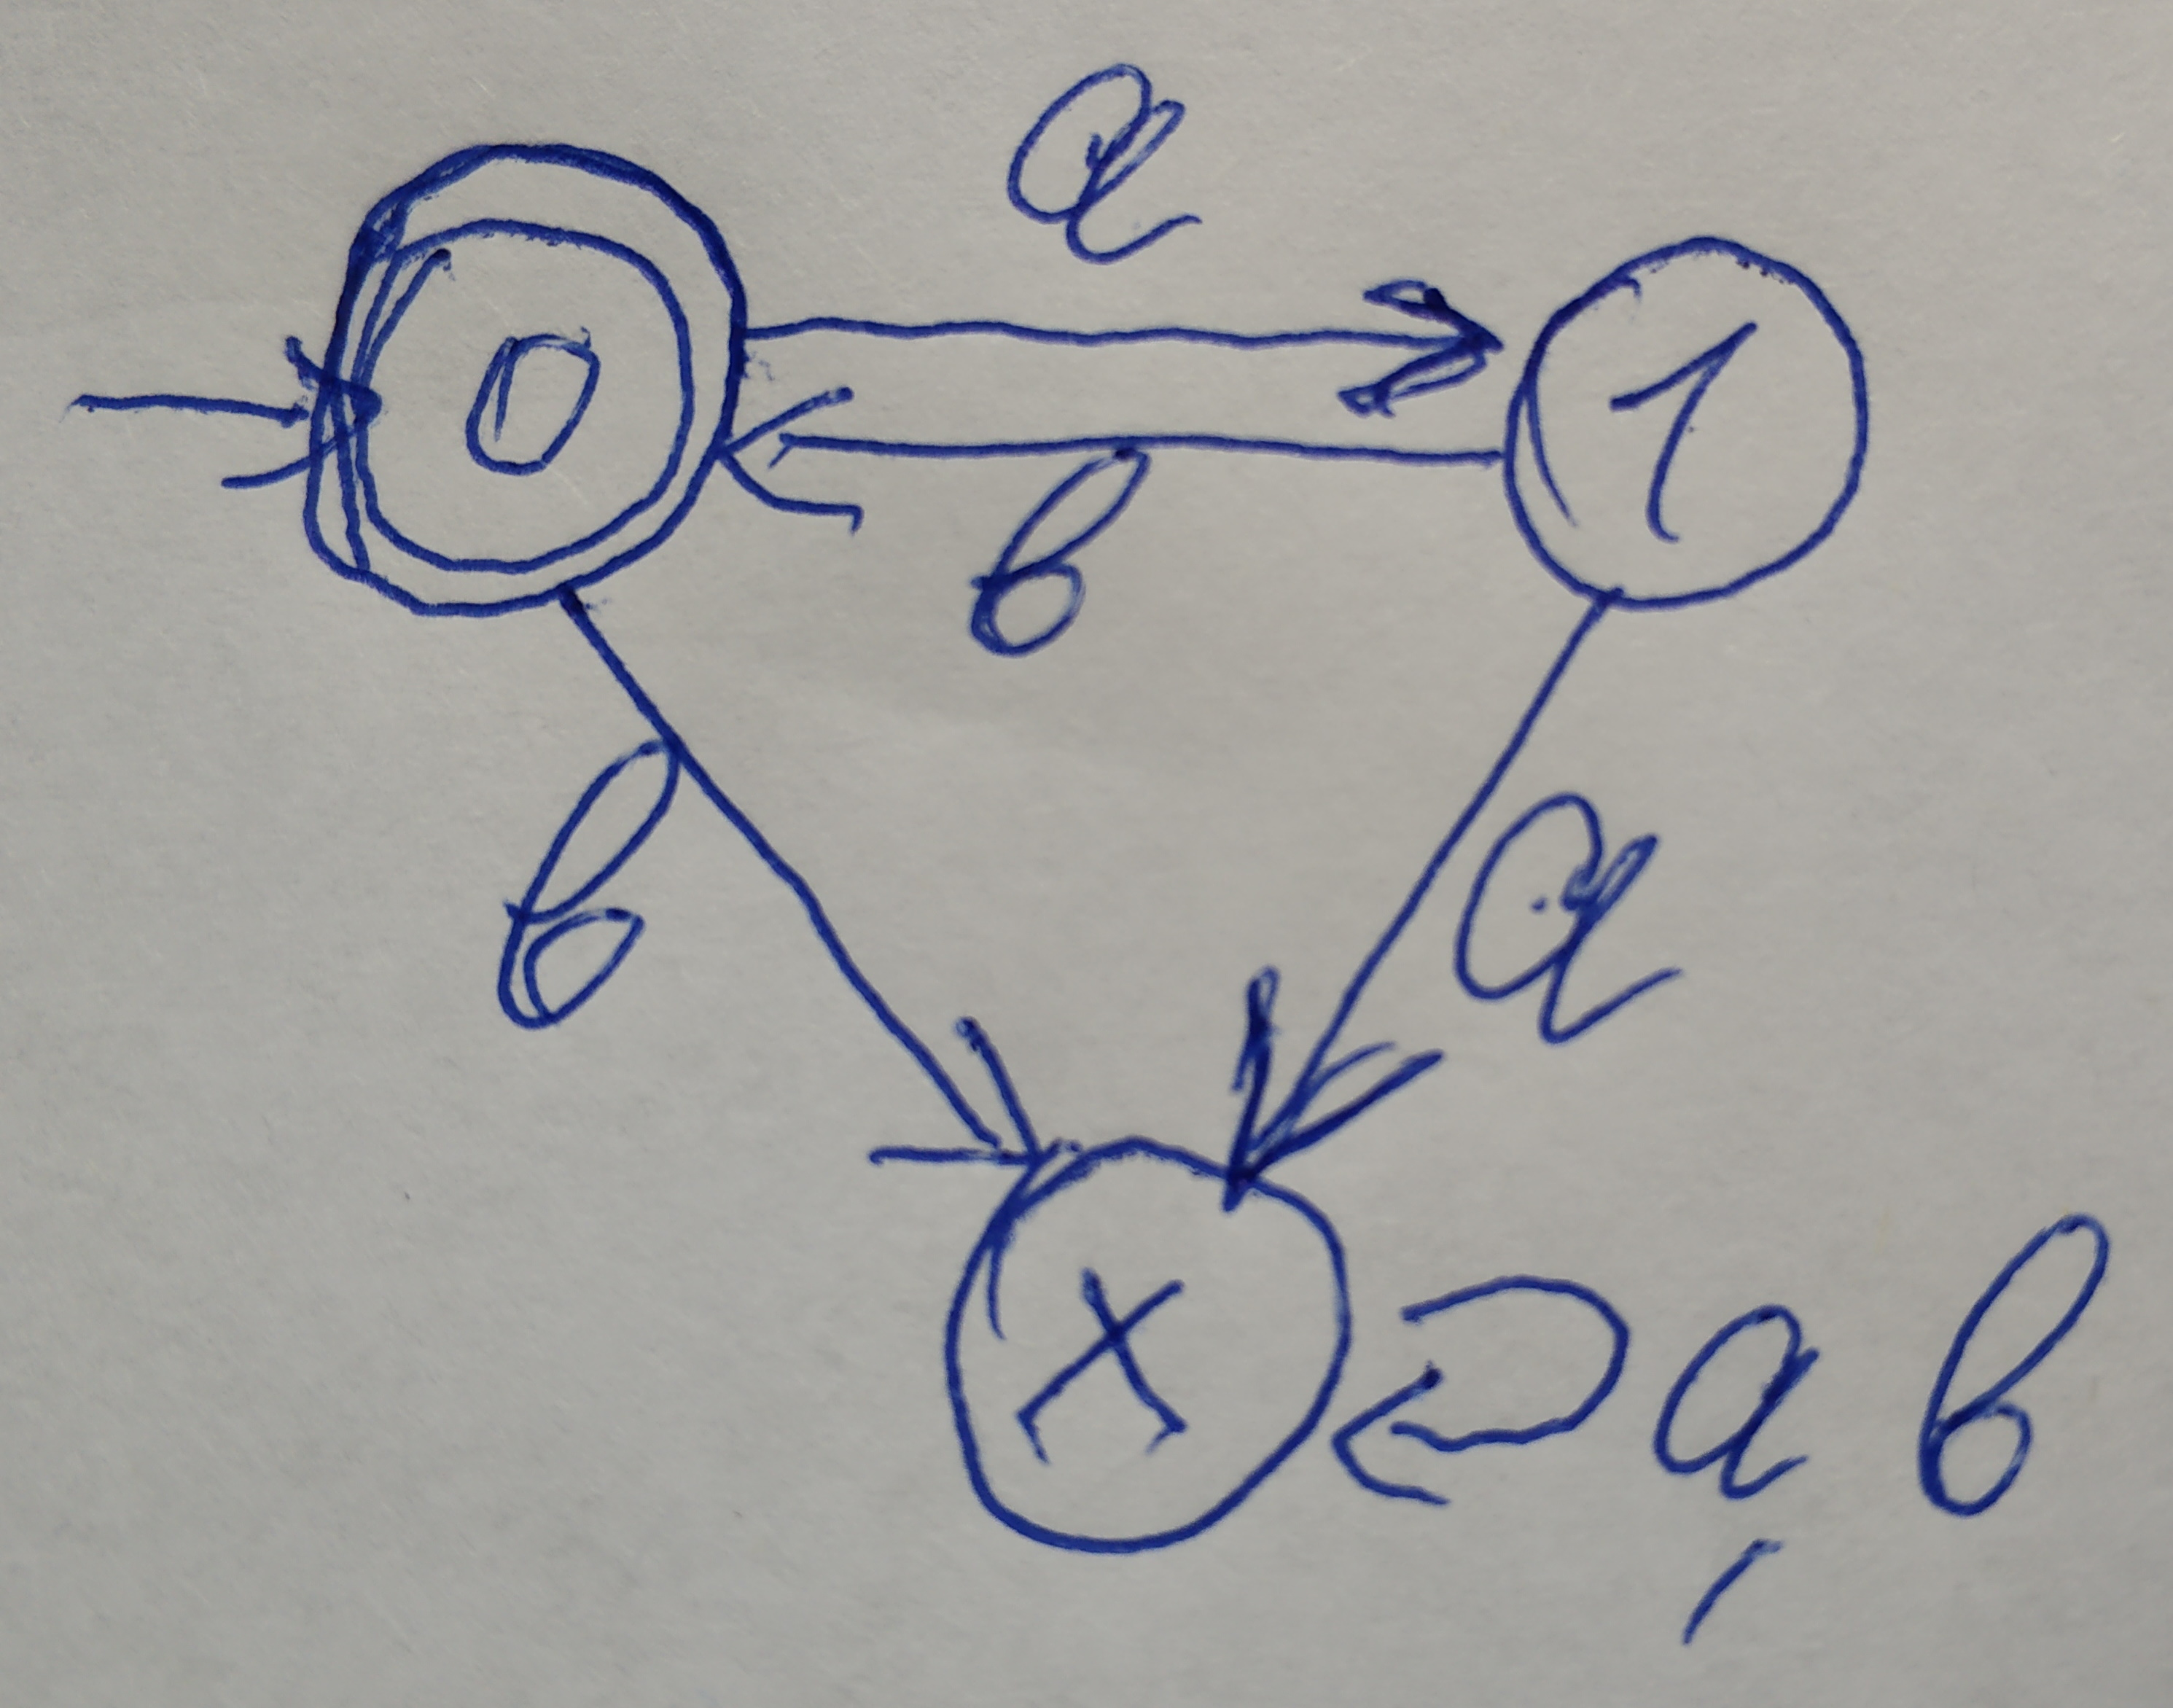
\includegraphics[height=5cm]{TI-HW-002-7.jpg}
        \end{figure}

        При этом язык $\lex(L) = \{a^n b^n\}_{n \in \NN}$. И при чём этот язык не является регулярным (было показано на лекции). Следовательно, утверждение неверно.
    \end{problem}
\end{document}